\subsubsection{Auktionsverfahren}
In dieser Arbeit betrachten wir eine sequentielle Rückwärtsauktion: Nacheinander findet für jede Baustellen eine Auktion statt, bei der die gesuchten Skilltypen einer Baustelle einzeln in ihrer benötigten Menge ausgeschrieben werden. Nun bieten die Agenten nacheinander auf die in gesuchten Skills. Sollte es auf ein einzelnes Gesuch keine Gebote geben, so ist die Auktion gescheitert, die Baustelle wird nicht fertiggestellt und ihr Erlös wird nicht ausgezahlt. In den Auktionen erhält das niedrigste Gebot den Zuschlag.

\begin{figure}
  \centering
  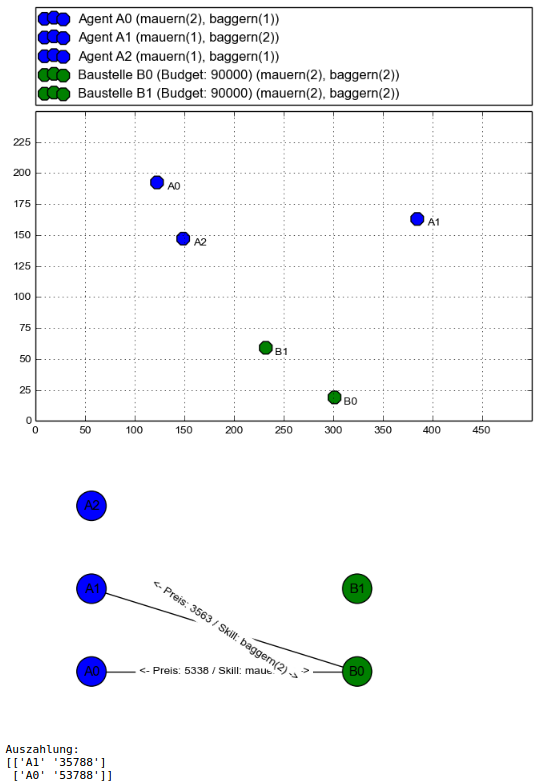
\includegraphics[width=0.45\textwidth]{example-srg.png}
  \caption{Ergebnis des Auktionsverfahrens.}
  \label{example-srg}
\end{figure}

Die Verteilung des Erlöses der Baustelle über die beliefernden Agenten orientiert sich an ihren Geboten: Zunächst wird jedem Agent der Gegenwert seines Gebotes ausgezahlt. Der darüber hinaus verbleibende Erlös der Baustelle wird auf die beliefernden Agenten aufgeteilt: Der Anteil eines Agenten entspricht dem Anteil ihres Gebotes an der Summe aller erfolgreichen Gebote für die Baustelle. In Abbildung \ref{example-srg} ist beispielhaft das Ergebnis für ein Szenario dargestellt.

\subsubsection{Ergebnisse}
Um eine vergleichende Untersuchung der Er\-lös\-ver\-tei\-lung zwischen Auktion und Shapley Value durchzuführen, generieren wir zunächst alle möglichen Szenarien mit der folgenden Charakteristik\footnote{Der Szenariengenerator ist Teil des für das Spiel implementierten GameFrameworks \cite{gitGame}}:

 Es existieren zwei Skills, zwei Baustellen und zwei Agenten. Die Auszahlungssumme der Baustellen ist immer $90000$ und die Kostenfunktion für alle Agenten und Skills ist abhängig von der Anzahl an Skills und der Distanz zwischen Agent und Baustelle: $f(Anzahl, \-Distanz)\- = (Anzahl/2+1)\-*Distanz\-+20*Anzahl$.

Die Agenten und Baustellen besitzen bzw. benötigen in den generierten Szenarien alle möglichen Kombinationen von diesen beiden Skills in der Quantität $1$ und $2$ bei den Skillkapazitäten und $1$ und $3$ bei den Skillgesuchen. Wir erzeugen so $4096$ Szenarien. 

\begin{figure}
  \centering
  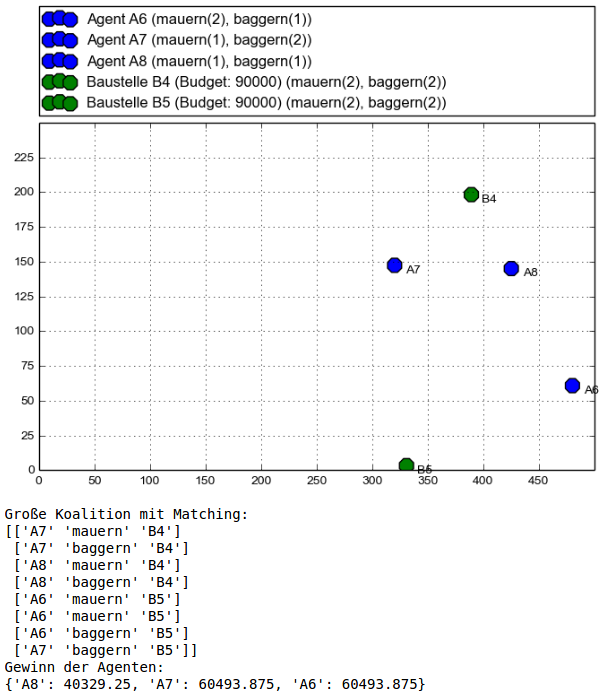
\includegraphics[width=0.45\textwidth]{example-shapley-value.png}
  \caption{Matching und Gewinnverteilung.}
  \label{example-shapley-value}
\end{figure}

Für diese Szenarien werden zunächst die Erlösverteilung nach dem Shapley Value und das dazugehörige Matching bestimmt \cite{gitShapley}. In Abbildung \ref{example-shapley-value} ist dazu das Ergebnis zu einem Beispielszenario zu sehen. Im zweiten Schritt wird die Auszahlung und die Zuordnung der Skills für alle Szenarien durch die Auktion bestimmt \cite{gitAuction}.

Die Ergebnisse der Simulationen weisen keine Überraschungen auf und werden deshalb nur kurz angedeutet: Die Zuweisungen des Auktionsverfahrens verläuft dank der niedrigeren Komplexitätsklasse deutlich schneller, die soziale Wohlfahrt (Summe der Gewinne aller Agenten) und damit auch die Anzahl der fertiggestellten Baustellen ist bei der Zuteilung über die große Koalition höher und der Unterschied zwischen dem Gewinn des Agenten mit dem niedrigsten Gewinn zu dem mit dem größten Gewinn ist beim Auktionsverfahren größer (Zuteilung weniger fair).

In der Abbildung \ref{results} sind diese Unterschiede in der Gewinnzuteilung zwischen Shapley Value und dem Auktionsverfahren dargestellt: Die jeweils über alle generierten Szenarien summierte soziale Wohlfahrt und der jeweilige summierte Gewinn des Agenten mit dem niedrigsten Gewinn und höchsten Gewinn im Szenario.

\begin{figure}
  \centering
  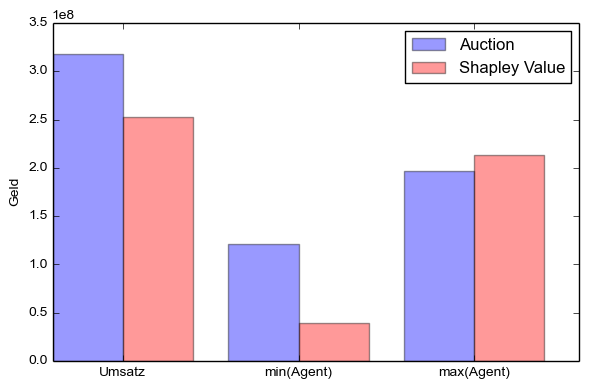
\includegraphics[width=0.4\textwidth]{results.png}
  \caption{Über alle simulierten Szenarien aggregierte Indikatoren.}
  \label{results}
\end{figure} 

